\section{Cambio de base}

\subsection{}

\begin{frame}\frametitle{Coordenadas}

\begin{ej}{\textbf{Ejemplo 1}}
	Halle los vectores de coordenadas del vector ${\color{blue}\mathbf{v}=(5,4)}$ en $\r^2$, respecto a las bases
	\[
		\mathcal{B} = \Big\{ \, \underbrace{(1,0)}_{\color{darkgreen}\mathbf{u}_1}, \ \underbrace{(0,1)}_{\color{darkgreen}\mathbf{u}_2} \, \Big\}
		\qquad \text{y} \qquad
		\mathcal{C} = \Big\{ \, \underbrace{(1,0)}_{\color{red}\mathbf{v}_1}, \ \underbrace{(1,2)}_{\color{red}\mathbf{v}_2} \, \Big\}.
	\]
\end{ej}

\vspace{-2mm}
\begin{columns}[c]
%	\onslide<+->{
		\begin{column}{0.6\textwidth}
			\begin{center}
				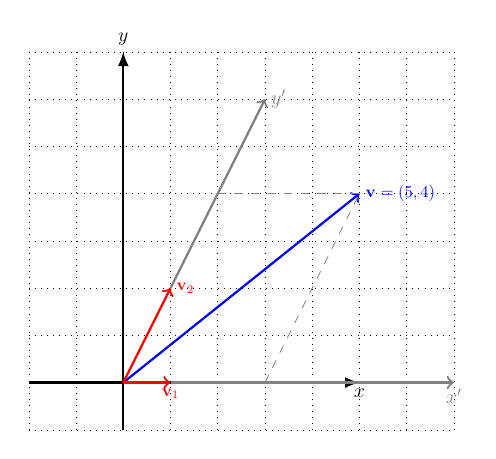
\begin{tikzpicture}[thick,scale=0.6, every node/.style={scale=0.6}]%[scale=.8,font=\scriptsize]
				\draw[help lines,black,dotted] (-2,-1) grid (7,7);
				\draw[thick,-latex] (-2,0) -- (5,0) node[below] {\large $x$};
				\draw[thick,-latex] (0,-1) -- (0,7) node[above] {\large $y$};
			%	\fill[color=green,draw] (0,0) circle (2pt); % node[below, left] {$(0,0)$};
			%	\fill[color=red,draw] (2,3) circle (2pt) node[above, right] {$(x_1,x_2)$};	
				%	\foreach \x in {-4,-3,-2,-1}{\draw[thick] (\x,.1)--(\x,-.1) node[below] {$\x$};}
				%	\foreach \x in {1,2,3,4}{\draw[thick] (\x,.1)--(\x,-.1) node[below] {$\x$};}
				%	\foreach \x in {1,2,3}{\draw[thick] (-.1,\x)--(.1,\x) node[right] {$\x$};}
				%	\foreach \x in {-1,-2,-3}{\draw[thick] (.1,\x)--(-.1,\x) node[left] {$\x$};}
				%	\node at (4.5,3.5) {\Large I}; \node at (-4.5,3.5) {\Large II}; 
				%	\node at (-4.5,-3.5) {\Large III}; \node at (4.5,-3.5) {\Large IV};
				\draw [color=blue,->] (0,0) -- (5,4);
				\fill[color=blue,draw] (5,4) node[above, right] {$\mathbf{v}=(5,4)$};
				\draw [color=red,->] (0,0) -- (1,0);
				\fill[color=red,draw] (1,0) node[below] {$\mathbf{v}_1$};
				\draw [color=red,->] (0,0) -- (1,2);
				\draw [color=gray,->] (1,0) -- (7,0);
				\fill[color=gray,draw] (7,0) node[below] {\large $x'$};
				\fill[color=red,draw] (1,2) node[above, right] {$\mathbf{v}_2$};
				\draw [color=gray,->] (1,2) -- (3,6);
				\fill[color=gray,draw] (3,6) node[above, right] {\large $y'$};
				\draw [line width=0.1mm,color=gray,dashed,-] (3,0) -- (5,4);
				\draw [line width=0.1mm,color=gray,dashed,-] (2,4) -- (5,4);
			%	\begin{scope}[rotate=20,draw=red]
			%		\draw[->] (0,0) -- (1,0)  node[right, text width=5em] {$X'$};
			%		\draw[->] (0,0) -- (1,2)  node[right, text width=5em] {$Y'$};
			%	\end{scope}
				\end{tikzpicture}
			\end{center}
	\end{column}
	%	}
	%\onslide<+->{
	%\pause
	
	\hspace{-1cm}
	\begin{column}{0.2\textwidth}
		\[
			\begin{array}{rlc}
				\left[ \mathbf{v} \right]_{\mathcal{B}} & = & ?\\[1cm]
				\left[ \mathbf{v} \right]_{\mathcal{C}} & = & ?
			\end{array}			
		\]	
	\end{column}
\end{columns}

\end{frame}

%%------------------------------------------------------------------------------------------------------

\subsection{}

\begin{frame}\frametitle{Coordenadas respecto a una  base no estándar}

\begin{ej}{\textbf{Ejemplo 2}}
	Considere en $\r^2$ las bases
	\[
	\mathcal{B} = \Bigg\{ \, \underbrace{ \left( \begin{array}{r}	-1 \\ 2 \end{array} \right) }_{\color{blue}\mathbf{u_1}}, \ 
	\underbrace{ \left( \begin{array}{r} 2 \\ -1 \end{array} \right) }_{\color{blue}\mathbf{u_2}} \, \Bigg\}
	\qquad \text{y} \qquad
	\mathcal{C} = \Bigg\{ \, \underbrace{ \left( \begin{array}{c}	1 \\ 0 \end{array} \right) }_{\color{blue}\mathbf{v_1}}, \ 
	\underbrace{ \left( \begin{array}{r}  1 \\ 1 \end{array} \right) }_{\color{blue}\mathbf{v_2}} \, \Bigg\}.
	\]
	Encuentre $\left[ \mathbf{x} \right]_{\mathcal{C}}$ dado que
	\[
	\left[ \mathbf{x} \right]_{\mathcal{B}} = 
	\left[
	\begin{array}{c}
	1\\
	3
	\end{array}
	\right].
	\]
\end{ej}
\textit{Solución.}

\end{frame}

%%------------------------------------------------------------------------------------------------------

\subsection{}

{\nologo
\begin{frame}\frametitle{Matriz de cambio de base}

\begin{defi}{\textbf{Definición 1}}\justifying
	Sean $\mathcal{B}=\{\mathbf{u}_1, \mathbf{u}_2, \hdots , \mathbf{u}_n \}$ y $\mathcal{C}=\{\mathbf{v}_1, \mathbf{v}_2, \hdots , \mathbf{v}_n \}$  bases para un espacio  vectorial $V$. A la matriz $n\times n$ cuyas columnas son los vectores coordenados
	\[
		\left[ \mathbf{u}_1 \right]_{\mathcal{C}}, \left[ \mathbf{u}_2 \right]_{\mathcal{C}}, \hdots, \left[ \mathbf{u}_n \right]_{\mathcal{C}}
	\]
	se le llama \textbf{\textit{matriz de cambio de base}} de $\mathcal{B}$ a $\mathcal{C}$ y se denota por $P_{\mathcal{C} \leftarrow\mathcal{B}}$. Es decir,	
	\[	
		P_{\mathcal{C} \leftarrow\mathcal{B}} =
		\left( 
			\begin{array}{c|c|c|c} \left[ \mathbf{u}_1 \right]_{\mathcal{C}} & \left[ \mathbf{u}_2 \right]_{\mathcal{C}} & \cdots & \left[ \mathbf{u}_n \right]_{\mathcal{C}}
			\end{array} 
		\right)
	\]
\end{defi}	

\vspace{0mm}

\begin{alertblock}{\textbf{Observación 1}}
	\begin{enumerate}
		\item[\labelname{$a$}] Piense en $\mathcal{B}$ como la base ``antigua'' y $\mathcal{C}$ como la base ``nueva''.
		\item[\labelname{$b$}] Las columnas de $P_{\mathcal{C} \leftarrow\mathcal{B}}$ son son precisamente los vectores 
		coordenados obtenidos al escribir los vectores de la base antigua en términos de los nuevos.
	\end{enumerate}
\end{alertblock}

\end{frame}
}

%%------------------------------------------------------------------------------------------------------

\subsection{}

{\nologo
\begin{frame}\frametitle{Matriz de cambio de base}

\begin{defi}{\textbf{Definición 1}}\justifying
	Sean $\mathcal{B}=\{\mathbf{u}_1, \mathbf{u}_2, \hdots , \mathbf{u}_n \}$ y $\mathcal{C}=\{\mathbf{v}_1, \mathbf{v}_2, \hdots , \mathbf{v}_n \}$  bases para un espacio  vectorial $V$. A la matriz $n\times n$ cuyas columnas son los vectores coordenados
	\[
	\left[ \mathbf{u}_1 \right]_{\mathcal{C}}, \left[ \mathbf{u}_2 \right]_{\mathcal{C}}, \hdots, \left[ \mathbf{u}_n \right]_{\mathcal{C}}
	\]
	se le llama \textbf{\textit{matriz de cambio de base}} de $\mathcal{B}$ a $\mathcal{C}$ y se denota por $P_{\mathcal{C} \leftarrow\mathcal{B}}$. Es decir,	
	\[	
	P_{\mathcal{C} \leftarrow\mathcal{B}} =
	\left( 
	\begin{array}{c|c|c|c} \left[ \mathbf{u}_1 \right]_{\mathcal{C}} & \left[ \mathbf{u}_2 \right]_{\mathcal{C}} & \cdots & \left[ \mathbf{u}_n \right]_{\mathcal{C}}
	\end{array} 
	\right)
	\]
\end{defi}	

\vspace{0mm}

\begin{prop}{\textbf{Propiedad 1}}
	\justifying
	Sean $\mathcal{B}=\{\mathbf{u}_1, \mathbf{u}_2, \hdots , \mathbf{u}_n \}$ y $\mathcal{C}=\{\mathbf{v}_1, \mathbf{v}_2, \hdots , \mathbf{v}_n \}$  bases para un espacio  vectorial $V$ y sea $P_{\mathcal{C} \leftarrow\mathcal{B}}$ la matriz de cambio 
	de base de $\mathcal{B}$ a $\mathcal{C}$. Entonces
	\begin{enumerate}
		\item[\labelname{$a$}] $P_{\mathcal{C} \leftarrow\mathcal{B}}\left[ \mathbf{x} \right]_{\mathcal{B}}=\left[ \mathbf{x} \right]_{\mathcal{C}}$ para todo $\mathbf{x}$ en $V$.
		\item[\labelname{$b$}] $P_{\mathcal{C} \leftarrow\mathcal{B}}$ es la única matriz que satisface la propiedad $(a)$.
		\item[\labelname{$c$}] $P_{\mathcal{C} \leftarrow\mathcal{B}}$ es invertible y $\left(P_{\mathcal{C} \leftarrow\mathcal{B}}\right)^{-1}=P_{\mathcal{B} \leftarrow\mathcal{C}}$		
	\end{enumerate}
\end{prop}	

\end{frame}
}

%%------------------------------------------------------------------------------------------------------

\subsection{}

{\nologo
\begin{frame}\frametitle{Matriz de cambio de base}

\begin{prop}{\textbf{Propiedad 1}}
	\justifying
	Sean $\mathcal{B}=\{\mathbf{u}_1, \mathbf{u}_2, \hdots , \mathbf{u}_n \}$ y $\mathcal{C}=\{\mathbf{v}_1, \mathbf{v}_2, \hdots , \mathbf{v}_n \}$  bases para un espacio  vectorial $V$ y sea $P_{\mathcal{C} \leftarrow\mathcal{B}}$ la matriz de cambio 
	de base de $\mathcal{B}$ a $\mathcal{C}$. Entonces
	\begin{enumerate}
		\item[\labelname{$a$}] $P_{\mathcal{C} \leftarrow\mathcal{B}}\left[ \mathbf{x} \right]_{\mathcal{B}}=\left[ \mathbf{x} \right]_{\mathcal{C}}$ para todo $\mathbf{x}$ en $V$.
		\item[\labelname{$b$}] $P_{\mathcal{C} \leftarrow\mathcal{B}}$ es la única matriz que satisface la propiedad $(a)$.
		\item[\labelname{$c$}] $P_{\mathcal{C} \leftarrow\mathcal{B}}$ es invertible y $\left(P_{\mathcal{C} \leftarrow\mathcal{B}}\right)^{-1}=P_{\mathcal{B} \leftarrow\mathcal{C}}$		
	\end{enumerate}
\end{prop}	

\vspace{0mm}

\begin{ej}{\textbf{Ejemplo 3}}
	Encuentre las matrices de cambio de base $P_{\mathcal{C} \leftarrow\mathcal{B}}$ y $P_{\mathcal{B} \leftarrow\mathcal{C}}$
	para
	\[
		\mathcal{B} = \left\{ 1, x, x^2 \right\} \qquad \text{y} \qquad \mathcal{C} = \left\{ 1+x, x+x^2, 1+x^2 \right\}.
	\]
	Luego encuentre el vector coordenado de $p(x)=1+2x-x^2$ respecto a $\mathcal{C}$.
\end{ej}
\textit{Solución.}

\end{frame}
}

%%------------------------------------------------------------------------------------------------------

\subsection{}

\begin{frame}\frametitle{Matriz de cambio de base}
	
	\begin{ej}{\textbf{Ejemplo 3}}
		Encuentre las matrices de cambio de base $P_{\mathcal{C} \leftarrow\mathcal{B}}$ y $P_{\mathcal{B} \leftarrow\mathcal{C}}$
		para
		\[
		\mathcal{B} = \left\{ 1, x, x^2 \right\} \qquad \text{y} \qquad \mathcal{C} = \left\{ 1+x, x+x^2, 1+x^2 \right\}.
		\]
		Luego encuentre el vector coordenado de $p(x)=1+2x-x^2$ respecto a $\mathcal{C}$.
	\end{ej}
	\textit{Solución.} (Continuación)
	
\end{frame}


%%------------------------------------------------------------------------------------------------------

\subsection{}

{\nologo
\begin{frame}\frametitle{Matriz de cambio de base}

\begin{prop}{\textbf{Propiedad 1}}
	\justifying
	Sean $\mathcal{B}=\{\mathbf{u}_1, \mathbf{u}_2, \hdots , \mathbf{u}_n \}$ y $\mathcal{C}=\{\mathbf{v}_1, \mathbf{v}_2, \hdots , \mathbf{v}_n \}$  bases para un espacio  vectorial $V$ y sea $P_{\mathcal{C} \leftarrow\mathcal{B}}$ la matriz de cambio 
	de base de $\mathcal{B}$ a $\mathcal{C}$. Entonces
	\begin{enumerate}
		\item[\labelname{$a$}] $P_{\mathcal{C} \leftarrow\mathcal{B}}\left[ \mathbf{x} \right]_{\mathcal{B}}=\left[ \mathbf{x} \right]_{\mathcal{C}}$ para todo $\mathbf{x}$ en $V$.
		\item[\labelname{$b$}] $P_{\mathcal{C} \leftarrow\mathcal{B}}$ es la única matriz que satisface la propiedad $(a)$.
		\item[\labelname{$c$}] $P_{\mathcal{C} \leftarrow\mathcal{B}}$ es invertible y $\left(P_{\mathcal{C} \leftarrow\mathcal{B}}\right)^{-1}=P_{\mathcal{B} \leftarrow\mathcal{C}}$		
	\end{enumerate}
\end{prop}	

\begin{alertblock}{\textbf{Observación 2}}\justifying
	Para encontrar $\left[ \mathbf{x} \right]_{\mathcal{C}}$ utilizando la propiedad 3$(a)$ no es necesario conocer explícitamente a
	la matriz de cambio de base
	\[	
	P_{\mathcal{C} \leftarrow\mathcal{B}} =
	\left( 
	\begin{array}{c|c|c|c} \left[ \mathbf{u}_1 \right]_{\mathcal{C}} & \left[ \mathbf{u}_2 \right]_{\mathcal{C}} & \cdots & \left[ \mathbf{u}_n \right]_{\mathcal{C}}
	\end{array} 
	\right).
	\]
	Si conocemos a $P_{\mathcal{B} \leftarrow\mathcal{C}}$ y a $\left[ \mathbf{x} \right]_{\mathcal{B}}$ podemos utilizar eliminación gaussiana así:
	\[	
	\left( 
	\begin{array}{c|c} P_{\mathcal{B} \leftarrow\mathcal{C}} & \left[ \mathbf{x} \right]_{\mathcal{B}}
	\end{array} 
	\right)
	\longrightarrow
	\left( 
	\begin{array}{c|c} I & \left(P_{\mathcal{B} \leftarrow\mathcal{C}}\right)^{-1}\left[ \mathbf{x} \right]_{\mathcal{B}}
	\end{array} 
	\right)
	\longrightarrow
	\left( 
	\begin{array}{c|c} I & P_{\mathcal{C} \leftarrow\mathcal{B}}\left[ \mathbf{x} \right]_{\mathcal{B}}
	\end{array} 
	\right)
	\]
\end{alertblock}

\end{frame}
}

%%------------------------------------------------------------------------------------------------------

\subsection{}

\begin{frame}%\frametitle{Matriz de cambio de base}

\begin{alertblock}{\textbf{Observación 2}}\justifying
	Para encontrar $\left[ \mathbf{x} \right]_{\mathcal{C}}$ utilizando la propiedad 3$(a)$ no es necesario conocer explícitamente a
	la matriz de cambio de base
	\[	
	P_{\mathcal{C} \leftarrow\mathcal{B}} =
	\left( 
	\begin{array}{c|c|c|c} \left[ \mathbf{u}_1 \right]_{\mathcal{C}} & \left[ \mathbf{u}_2 \right]_{\mathcal{C}} & \cdots & \left[ \mathbf{u}_n \right]_{\mathcal{C}}
	\end{array} 
	\right).
	\]
	Si conocemos a $P_{\mathcal{B} \leftarrow\mathcal{C}}$ y a $\left[ \mathbf{x} \right]_{\mathcal{B}}$ podemos utilizar eliminación gaussiana así:
	\[	
	\left( 
	\begin{array}{c|c} P_{\mathcal{B} \leftarrow\mathcal{C}} & \left[ \mathbf{x} \right]_{\mathcal{B}}
	\end{array} 
	\right)
	\longrightarrow
	\left( 
	\begin{array}{c|c} I & \left(P_{\mathcal{B} \leftarrow\mathcal{C}}\right)^{-1}\left[ \mathbf{x} \right]_{\mathcal{B}}
	\end{array} 
	\right)
	\longrightarrow
	\left( 
	\begin{array}{c|c} I & P_{\mathcal{C} \leftarrow\mathcal{B}}\left[ \mathbf{x} \right]_{\mathcal{B}}
	\end{array} 
	\right)
	\]
\end{alertblock}

\begin{ej}{\textbf{Ejemplo 4}}
	Encuentre el vector de coordenadas de $\mathbf{x}=(1,2,-1)$ en $\r^3$, respecto a la base
	\[
	\mathcal{C} = \Big\{ \, (1,0,1), \ (0,-1,2), \ (2,3,-5) \, \Big\}.
	\]
\end{ej}
\textit{Solución.}

\end{frame}

%%------------------------------------------------------------------------------------------------------

\subsection{}

{\nologo
\begin{frame}\frametitle{Matriz de cambio de base por medio de eliminación de Gauss-Jordan}

\vspace{-2mm}
\begin{prop}{\textbf{Propiedad 2}}
	\justifying
	Sean $\mathcal{B}=\{\mathbf{u}_1, \mathbf{u}_2, \hdots , \mathbf{u}_n \}$ y $\mathcal{C}=\{\mathbf{v}_1, \mathbf{v}_2, \hdots , \mathbf{v}_n \}$  bases para un espacio  vectorial $V$. Sean
	\[
	B = \left( 
	\begin{array}{c|c|c|c} \left[ \mathbf{u}_1 \right]_{\mathcal{E}} & \left[ \mathbf{u}_2 \right]_{\mathcal{E}} & \cdots & \left[ \mathbf{u}_n \right]_{\mathcal{E}}
	\end{array} 
	\right)
	\]
	y 
	\[
	C = \left( 
	\begin{array}{c|c|c|c} \left[ \mathbf{v}_1 \right]_{\mathcal{E}} & \left[ \mathbf{v}_2 \right]_{\mathcal{E}} & \cdots & \left[ \mathbf{v}_n \right]_{\mathcal{E}}
	\end{array} 
	\right),
	\]
	donde $\mathcal{E}$ es cualquier base para $V$. Entonces al aplicar eliminación de Gauss-Jordan a la matriz aumentada $(\ C\ |\ B\ )$, se obtiene
	\[	
	\left( 
	\begin{array}{c|c} C & B
	\end{array} 
	\right)
	\longrightarrow
	\left( 
	\begin{array}{c|c} I & P_{\mathcal{C} \leftarrow\mathcal{B}}
	\end{array} 
	\right).
	\]
\end{prop}	

\begin{alertblock}{\textbf{Observación 3}}
	Si $\mathcal{E}$ es una base canónica, la propiedad 2 es muy fácil de usar porque en tal caso
	\[
		B = P_{\mathcal{E} \leftarrow\mathcal{B}} \qquad \text{y} \qquad 
		C = P_{\mathcal{E} \leftarrow\mathcal{C}}
	\]
	son muy fáciles de calcular.
\end{alertblock}

\end{frame}
}

%%------------------------------------------------------------------------------------------------------

\subsection{}

\begin{frame}\frametitle{Matriz de cambio de base por medio de eliminación de Gauss-Jordan}

%\begin{prop}{\textbf{Propiedad 2}}
%	\justifying
%	Sean $\mathcal{B}=\{\mathbf{u}_1, \mathbf{u}_2, \hdots , \mathbf{u}_n \}$ y $\mathcal{C}=\{\mathbf{v}_1, \mathbf{v}_2, \hdots , \mathbf{v}_n \}$  bases para un espacio  vectorial $V$. Sean
%	\[
%	B = \left( 
%	\begin{array}{c|c|c|c} \left[ \mathbf{u}_1 \right]_{\mathcal{E}} & \left[ \mathbf{u}_2 \right]_{\mathcal{E}} & \cdots & \left[ \mathbf{u}_n \right]_{\mathcal{E}}
%	\end{array} 
%	\right)
%	\]
%	y 
%	\[
%	C = \left( 
%	\begin{array}{c|c|c|c} \left[ \mathbf{v}_1 \right]_{\mathcal{E}} & \left[ \mathbf{v}_2 \right]_{\mathcal{E}} & \cdots & \left[ \mathbf{v}_n \right]_{\mathcal{E}}
%	\end{array} 
%	\right),
%	\]
%	donde $\mathcal{E}$ es cualquier base para $V$. Entonces al aplicar eliminación de Gauss-Jordan a la matriz aumentada $(\ C\ |\ B\ )$, se obtiene
%	\[	
%	\left( 
%	\begin{array}{c|c} C & B
%	\end{array} 
%	\right)
%	\longrightarrow
%	\left( 
%	\begin{array}{c|c} I & P_{\mathcal{C} \leftarrow\mathcal{B}}
%	\end{array} 
%	\right).
%	\]
%\end{prop}	

\begin{ej}{\textbf{Ejemplo 5}}
	Encuentre la matriz de cambio de base de $\mathcal{B}$ a $\mathcal{C}$ para las siguientes bases de $\r^3$:
	\[
	\mathcal{B} = \Big\{ (6,3,3), (4,-1,3), (5,5,2) \Big\} 
	\quad \text{y} \quad
	\mathcal{C} = \Big\{ (2,0,1), (1,2,0), (1,1,1) \Big\}.
	\]
\end{ej}
\textit{Solución}.

\end{frame}

%%------------------------------------------------------------------------------------------------------

\subsection{}

\begin{frame}%\frametitle{Coordenadas respecto a la base canónica (estándar)}

%\begin{prop}{\textbf{Propiedad 2}}
%	\justifying
%	Sean $\mathcal{B}=\{\mathbf{u}_1, \mathbf{u}_2, \hdots , \mathbf{u}_n \}$ y $\mathcal{C}=\{\mathbf{v}_1, \mathbf{v}_2, \hdots , \mathbf{v}_n \}$  bases para un espacio  vectorial $V$. Sean
%	\[
%	B = \left( 
%	\begin{array}{c|c|c|c} \left[ \mathbf{u}_1 \right]_{\mathcal{E}} & \left[ \mathbf{u}_2 \right]_{\mathcal{E}} & \cdots & \left[ \mathbf{u}_n \right]_{\mathcal{E}}
%	\end{array} 
%	\right)
%	\]
%	y 
%	\[
%	C = \left( 
%	\begin{array}{c|c|c|c} \left[ \mathbf{v}_1 \right]_{\mathcal{E}} & \left[ \mathbf{v}_2 \right]_{\mathcal{E}} & \cdots & \left[ \mathbf{v}_n \right]_{\mathcal{E}}
%	\end{array} 
%	\right),
%	\]
%	donde $\mathcal{E}$ es cualquier base para $V$. Entonces al aplicar eliminación de Gauss-Jordan a la matriz aumentada $(\ C\ |\ B\ )$, se obtiene
%	\[	
%	\left( 
%	\begin{array}{c|c} C & B
%	\end{array} 
%	\right)
%	\longrightarrow
%	\left( 
%	\begin{array}{c|c} I & P_{\mathcal{C} \leftarrow\mathcal{B}}
%	\end{array} 
%	\right).
%	\]
%\end{prop}	

\begin{ej}{\textbf{Ejemplo 6}}
	En $P_2$,
	
	\vspace{-2mm}
	\[
	\left[ p(x) \right]_{\mathcal{B}} = 
	\left[
	\begin{array}{c}
	2\\
	1\\
	3
	\end{array}
	\right],
	\qquad \text{donde} \qquad
	\mathcal{B} = \Big\{ \, 6-x, \ 3x,\ x^2-x-2 \, \Big\}.
	\]
	Escriba a $p(x)$ en términos de la base $\mathcal{C} = \Big\{ \, 2, \ -4+x,\ x+x^2 \, \Big\}$.
	
\end{ej}
\textit{Solución}.

\end{frame}